%!TEX root=thesis.tex
\chapter{Implementation}
% Command - B = compile

\section{Working Environment Setup} 

We use a server host provider service (Meebox), which comes with a package that supports php development, offers access to MariaDB 10.0.27, and includes phpMyAdmin as database management tool. On top of these it provides SSH Access and SSL Management.\\

I have suggested Github as our Version Control System, and learned Slack as the company's favorite Communication Management Tool. 
We have created a separate environment for testing and for production and for this purpose we have created a database for each environment. All the local changes are tested on the test database which is on the server.\\

I have chosen as IDE (Integrated Development Environment) PHPStorm, which is Jetbrains product for php development. Our main team tasks management tool was Trello, where we split tasks in categories and constantly prioritized our workflow.

\section{Front-End}

We have opted for a minimalistic, simple design for our beta version, as a strategy to iteratively develop it while testing its usability with end-users. This approach facilitates later integration of graphics. The trademarks of our front-end user interface design are: responsiveness, minimalist and intuitive, kids-friendly.\\

\subsection{Programming Languages} 

On front-end I mostly use Javascript Jquery libraries. Apart from substantially compressing the code in fewer lines, JQuery is also the most broswer-friendly. It does not need Adobe Flash plug-in to be interpreted by the browser, meaning it is readable in any browser. (http://www.javaworld.com/article/2078613/java-web-development/6-reasons-you-should-be-using-jquery.html)
\\

I use SCSS as a preprocessor programming language, to facilitate better standardization and omogenity of UI components. Jetbrains PHPStorm comes with a File Watcher, a transpiler tool for SCSS that facilitated its integration.\\

As a working practice I keep the mark-up language separated from Javascript as much as possible. I use small modules of Javascript code, usually a Javascript file corresponding to an UI component.
The application also has a dedicated layout folder, that comprises the layout elements common to all or some of the application pages. 

\subsection{UI Framework} 

The front-end framework we use is Bootstrap Twitter 3.3.6. We have settled on Boostrap after analysing pros and cons of alternative frameworks.
Although frameworks like Foundation, Semantic UI, Material Design, Ulkit have some competitive features, Boostrap won by having some unbeatable advantages.\\

It corresponds to one of our core design principles: responsiveness. It exceeds other frameworks by its stated attention towards resposiveness and mobile-friendliness.
Bootstrap is still regarded as the most popular front-end framework, with large community support and consequenlty with rich documentation and resources: articles and tutorials, third-party plug-ins and extensions, theme builders.\\

I also prefer Boostrap beacause of its level of specificity. Being more generic than other frameworks that tend to have higher-level specificity, its minimal style framework is easier to customise. I consider it is more practical to add up styling rules than overwriting existing ones. 
(Ref: https://www.sitepoint.com/5-most-popular-frontend-frameworks-compared/)\\

A good framework needs to level up constantly with the latest web technologies, especially with regards to mobile. Bootsrap does that, being constantly under active development. It also has a generous browser support.\\	

Some of the other frameworks have some very competitive features. Semantic UI has some extra unique UI components and outperforms Boostrap as a very friendly, semantic language. Its overall structure of the framework and the naming conventions, in terms of clear logic and semantics of its classes has a clear vantage point. It prounds itself with a scalable and modular architecture for CSS as main property.\\

Frameworks such as Semantic UI and Foundation also outweight others by a unique, rich pallette of UI components.
YOOtheme distinguishes itself with a better GUI Customizer. It offers a flexible and powerful customization mechanism, either manually or via its GUI customizer.
Regarding the spectrum of browser support, Boostrap finds itself a step behind Foundation.\\


\section{Back-End}

\subsection{Programming language} 

I have built the application using the scripting language PHP as server-side choice. I believe it is a reliable choice, as PHP has steadily been one of the most widely used developing language for web applications. It is commonly known for its portability and it is supported by the highest number of web server hosting providers. 
PHP is widely backed by large programming communities and it is open source, which assures a steady development and a solid community commitment in stabilizing it.\\ 

PHP is also known for its flexibility/resilience. It it portable on all major operating systems, can function both as a module or a CGI processor and has support on a wide range of web servers. PHP  holds up both procedural and object-oriented (OOP) programming paradigms, and has compatibility with a vast collection of databases.\\ 

For relational database management system (RDMS) I have opted for MySql. PHP can use mainstream MySQLLi and also provides an abstraction layer through PDO, which I have made use of.

\subsection{RDMS} 

PDO stands for PHP Data Objects. It provides a data-access abstraction layer, using a unified API, which is a lean, consistent way to access databases regardless of the database. This increases the portability of our code, if we want to change the database we operate with.\\

One core advantage of PDO over MySQLi lyes in its database driver support. PDO upholds around 12 different drivers, opposed to MySQLi, which supports MySQL only. This fact has implications for further software changes, as using PDO makes it facile to transfer to a different database.\\  

The abstraction layer PHP offers in interaction with the database through PDO optimises the program execution and maximises security measurements.
The performance is boosted by the use of Prepared Statements, which allows the parsing and execution of a query only once. The queries are sent only once to the database, where they wait for the parameters. The bandwidth to the server is minimalized through the use of Binding Parameters, which are sent independently to the query waiting on the db.\\ 

The second advantage of employing PDO is the layer of security it provides. It is designed to shield against one of the most invasive forms of security breaches: SQL injections. The parameters sent in the query are transmitted later than the query commands using a different protocol. They are scrunitized with security filters through these protocols.\\ 

In the design of our database, we have used all types of relational raports between tables. One-to-one relationship model is predominent, followed by one-to-many pattern. 
The many-to-many relationship is used in merging data between tables such Members-Projects, Projects-Steps, Members-Achievements, Members-Activities, Members-Quizzes, Members-Comments.
I describe the database design using the following Entity Relation Diagram. I have used a coloristic relation map to differentiate the types of dependency between tables and data.
[Sceenshot DB Entity-Relation]\\


\section{Application Architecture and Design Principles}

I will exemplify the application architecture and the design principles by presenting the interactions of one of the projects main modules: the Projects section. The following diagram shows the organization and dependencies between the files of the module. [Figure 3.2]

\begin{figure}
\includegraphics[width=1\linewidth]{images/ProjectsDependencies.png}
\caption{File Dependencies Projects.}
\label{fig:file_dependencies_projects}
\end{figure}

\subsection{Design Principles}

I have designed my code around few pillarstone principles: separation of concerns, DRY (Do Not Repeat Yourself) and modularity (reusable components). Separation of concern principle is commonly associated with the MVC architecture design pattern. Although I do not employ a standard MVC framework, I have structured the composition of the code by applying MVC patterns, by striving to preserve a neat separation between the business logic and the view.\\ 

On Client-side I have separated the plain presentation from functionality, by keeping the the mark-up language from javascript in separate files. For readability purposes, I structured the front-end code in smaller separate files, so any major UI component is represented by a distinct file.\\ 

Because I make frequent use of Ajax calls, steadilyI have decided to dedicate a separate file where I have modelled an ajax API, that defines all ajax calls functions used throughout Projects (ajaxProjectsAPI.js). Doing so, I gain readibility of the code, by having a javascript file that only deals with the actual ajax calls, and the other javascript file only displaying the data in the view. The next advantage it promotes is modularity. Having a universal ajax API for the Projects module, I centralize all the ajax calls under reusable functions, that are accessible from any file of the module and even to other modules. This way, I can use same ajax function when needed and forestall redundancy of code.
For example,(as shown in the diagram) the ajaxUploadFile function is called from different js files of the same module/folder, or can be called from other modules, anywhere in the system.(or change example)\\ 

I'll describe the design of the AJAX API. It has 2 central generalized Ajax calls functions: postAjaxCall and postAjaxCallSendDictParams. postAjaxCall function sends as data only one parameter, while the other takes a dictionary for sending a couple of arguments to the server.
Both functions take the following arguments: the server-side endpoint they are sending data to, the data to be sent (name of the action and parameters), and a function that will be executed (in javascript) if the ajax call has been successful. [See Figure XX] \\ 

\begin{figure}
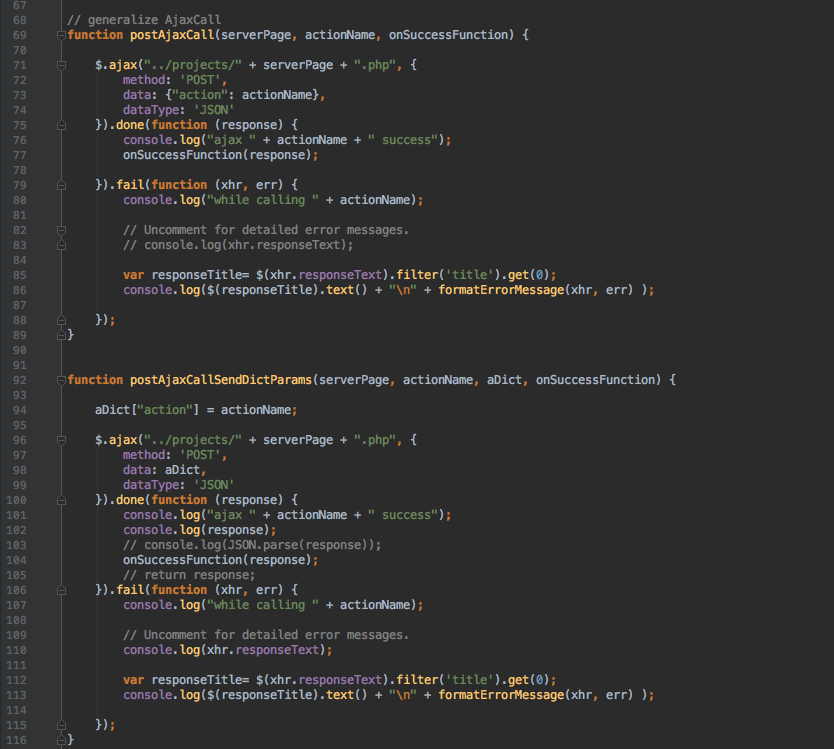
\includegraphics[width=1\linewidth]{images/GeneralisedAjaxCallsAPI.png}
\caption{Generalised Ajax Calls API.}
\label{fig:gen_ajax_calls}
\end{figure}

All the other functions of the Ajax API are calling one of the 2 generalized functions, depending on the amount of data they send. 
I have payed attention at functions naming conventions, as part of my clean code effort strategy. Consequently, these functions are suggestively named by the type of action they perform on the back-end, their name having in composition the name of action parameter sent as data.[See Figure XX] \\

\begin{figure}
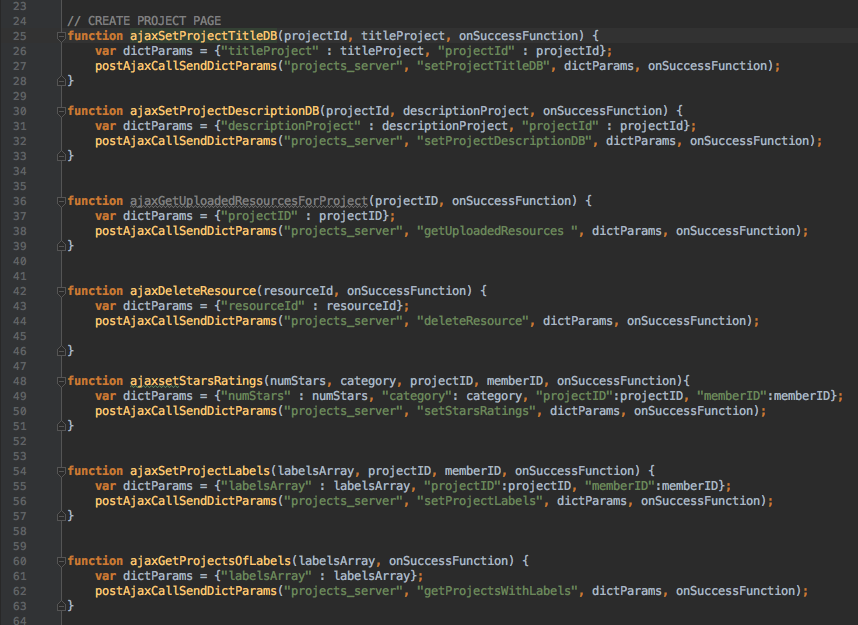
\includegraphics[width=1\linewidth]{images/AjaxProjectsAPI.png}
\caption{Ajax Projects API.}
\label{fig:ajax_projects_API}
\end{figure}


The Ajax API is for my application what the Controller is for the MVC pattern. It acts as an intermediary between the server-side(business logic) and the front-end(view). Basically, it solicits data from the server, takes the result data and transfers it to the view, without processing it in any way.\\  

Having the Ajax calls isolated, the other javascript files are left to perform the display of data. I encapsulate the display mechanism in functions. 
I have created distinctive functions for each display demand of data in the interface. By doing so, display functions can be reused by other functions and the readibility of the code is increased. Moreover, it increases modularity and it facilitates easy future changes or integration of new components in the UI.
Commonly, a javascript function in the system will call one or more ajax functions and will pass it as argument a display function, like in the next snippet example.\\ 

\begin{figure}
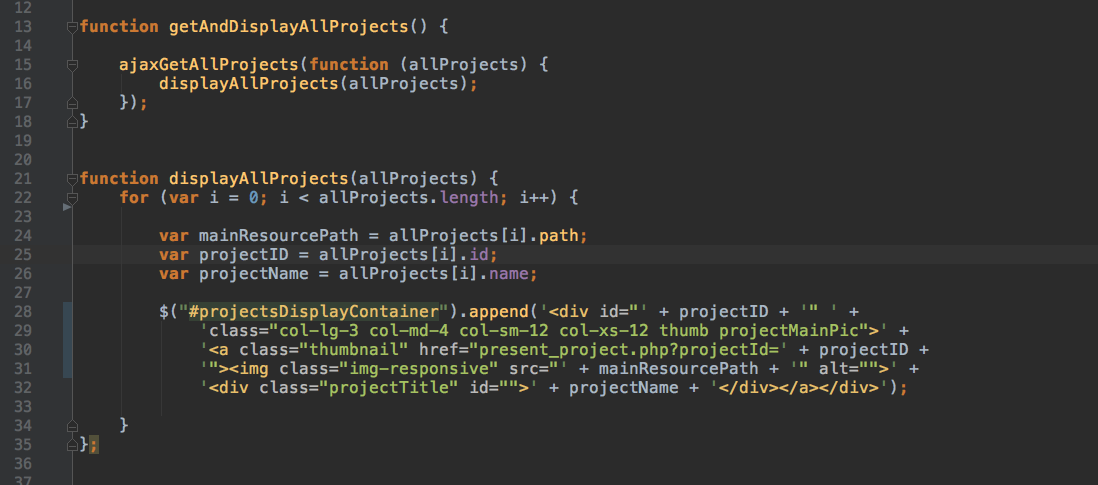
\includegraphics[width=1\linewidth]{images/JavascriptFunction.png}
\caption{Javascript Typical Function Design.}
\label{fig:javascript_function}
\end{figure}

On Server-side, I have organised the API in 2 main files: projects\_functions.php and projects\_server.php. In projects\_server.php are all functions and the database requests/queries called through the Ajax API that are sent to the Data Server, while in projects\_functions all the other functions, associated with the Web Server requests.
Besides the two endpoints, I separate the back-end functions for self-contained actions in independent files, like uploading media resources in upload.php, adding the steps for the project in addSteps.php and uploading steps in upload\_steps.php.\\

Another clean code principle I have developed while designing the application is trying to perform as much processing of data as possible on the back-end and in queries, obtaining as clear-cut data as needed in front-end (with less functionalities in javascript). 


\subsection{Client-Server Architecture}

The Front-end API is represented by the functions responsible with the data display which are organised in the js files and the ajax functions. \\

I make a formal distinction between functions which are both called and executed on server-side and those which are actually called on client side in javascript, by keeping them in separate files/by refering to them in 2 distinct end-points. The ones on the client are passing through the AjaxProjectsAPI and are executed in projects\_server.php.The functions that are both called and executed on server are collected/defined in projects\_functions.php.
I have decided which of the two function execution model to use in each situation, by analysing the on the amount of data requested and the probability of future reuse of the inquired data.

In the following I will present the client-server architecture of the application by analysing the interactions derived from each page of the projects module. 

\subsection{All Projects Page}
\url{/projects/index.php}

This page displays all existent projects and a collection of labels that users can select for filtering and searching the projects by categories. \\

The data of the category tags is retrieved through the getAllProjectsLabels() of the projects\_functions.php endpoint, which is displayed directly in the index.php.\\

For the category filter tags system, I use Ajax in retrieving and displaying the projects that result in labels selection. I have prefered to dynamically update the page with the selected projects rather than refresh the page, as it was more facile to hide the unselected projects in javascript than updating the page with the previously selected labels. This way, after the filter event is triggered, only the projects section is dynamically changed, the selected labels remaining unchanged.\\

All these interactions are described in Figure 3.4.

The page also gives the user the possibility of adding a new project. The 'Add New Project' button will redirect the user to the following url:
\url{projects/edit\_project.php?projectId}. In the background, the click event actually links to \url{projects/create\_project.php}, from where the user is redirected to the edit page. I will explain the logic of this process in the 'Create New Project Page' description.

\begin{figure}
\includegraphics[width=1\linewidth]{images/ArchitectureAllProjects.png}
\caption{Architecture All Projects.}
\label{fig:architecture_all_projects.}
\end{figure}

\subsection{Create New Project Page}
\url{projects/create\_project.php}

create\_project.php has only a mediating and rerouting function between index.php and edit\_project.php. Before saving the edited information of a newly created project, we first need an entry of the new project in the db. 
In create\_project.php, we insert a new project in the database with no other data than its id. Then we extract the id, sending it as an argument and redirecting to edit\_project.php?{projectID}. See Figure 3.7.

\begin{figure}
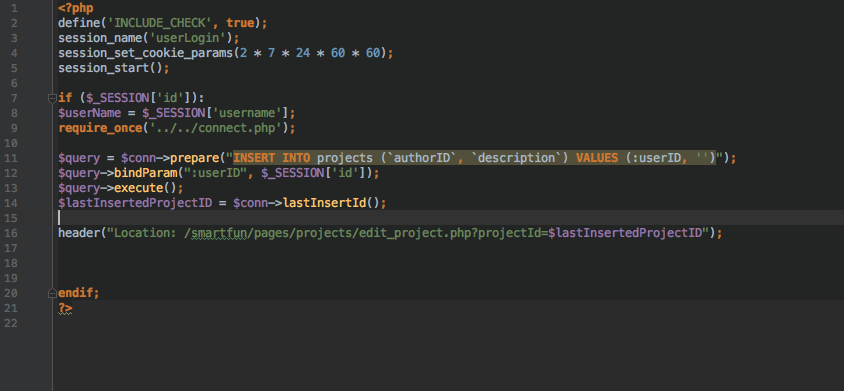
\includegraphics[width=1\linewidth]{images/CreateProjectPage.png}
\caption{Create Project Page.}
\label{fig:create_project.}
\end{figure}


In the end, creating a new project and editing an existing one, both happen in the edit page, as we'll subsequently see.

\subsection{Edit Project Page}
\url{/projects/edit\_project.php/{projectID}}

The page is accessed in two situations. One instance is when the user creates a new project, case in which it receives the id of the new project through a GET protocol from the create\_project.php.
The other is when the project was already created and the user only expects to edit the information. This case is accessed from the present\_project page. At the moment the editing of an existing project is open only to administrators. Their access to edit the project is done from the same project presentation page available to all users, through an event which is visible only the the admins of the system, as shown in Figure 3.8.\\

\begin{figure}
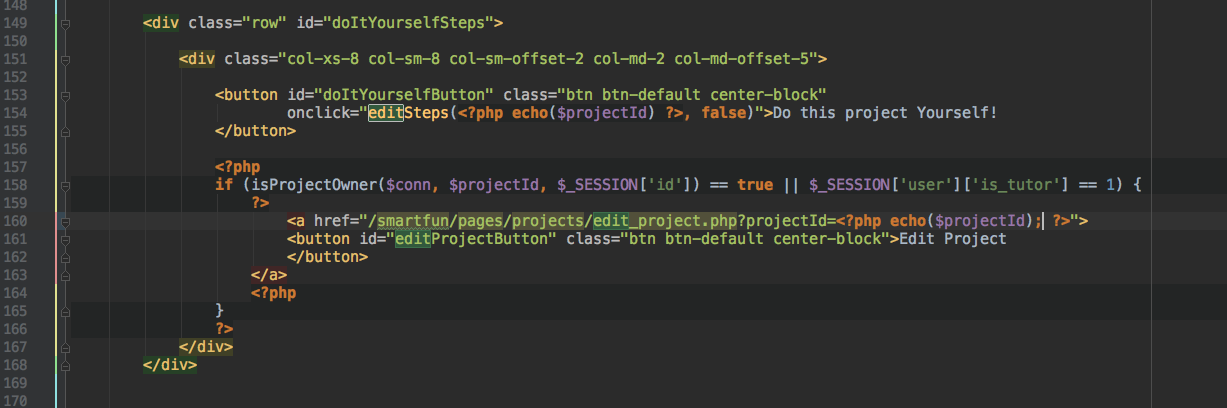
\includegraphics[width=1\linewidth]{images/edit.png}
\caption{Edit Project.}
\label{fig:edit_project.}
\end{figure}	

Editing projects connects to both main endpoints: the projectsDataServerAPI.php and the projectsAPI.php. The projectsAPI.php returns information about the editing project: title, description, uploaded media resouces, materials list. The functions contained in this endpoint are depicted in figure XX. \\	

The projectsDataServerAPI.php endpoint processes the edited information of the project sent to the server through the Ajax API. The Ajax functions are called by triggered events defined in projects.js, projects\_equipment.js and addSteps.js files, all included in edit\_project.php.\\

A core feature of the projects section is the presentation of the project in a succession of steps. The javascript functions of editing these steps are initialized in addSteps.js.
Although it is a self-sustaining solid feature, instead of dedicating a new page for editing the steps, we opted for displaying it within the edit\_project.php page, in a full-page pop-up element. The content of each step is modified dynamically inside same markup elements. Javascript functions used in addSteps.js: showStepPanel(), addStep(), deleteStep(), loadProjectProgress(), updateProgresBar().\\

Functions of the ajaxProjectsAPI.js that connect the editing projects front-end with the endpoint projectsDataServerAPI.php:  ajaxSetProjectTitleDB, ajaxSetProjectDescriptDB. 

 \subsection{Present Project}
\url{/projects/present\_project.php/{projectID}}	

Gets information from web server about the requested project.
Besides the project description and a carrousel with project pictures, it includes a few dynamic components the user can interact with. present\_project.php include a number of javascipt files, each correspondent to one of these UI components.\\

One component is the Stars Rating System, where users can evaluate the project by voting on a 5 stars scale on criterias denoting project's level of: difficulty, fun and general. In stars\_ratings.js I define the functions that show interactions with the ratings system. Each criteria voted in the system is individually updated in the database through a concurrent Ajax.\\

Second dynamic component is Projects Labels Section, where users can participate in adding descriptive tags about the project. In the current version, users can add up any labels that are yet non-existant. We have two alternative scenarios for dealing with the obvious problems this approach raises (too many user entries, unrelevant of inapropriate label names). We consider implementing a filter of the labels as a feature in the admin panel, or alternatively we could leave the feature only for admin use. \\

The Project Equiments Section is the third component users can interact with. This component lists all the needed equipments for carrying out the project. Users can check the items they already possess or can send to basket items they would need and like to buy. The event handling for the equipments is encapsulated in projects\_equipment.js. \\

Users can exchange ideas through the Comments Section, which can be monitored and managed(edited/deleted) by admins. comments.js processes the events linked to users comments.\\

Users can find a detailed description of how to do themselves the project in the Steps Section. Steps represent a tutorial about building the project. We use the same UI component for displaying the steps as for editing them, by using control structures and javascript hide and display functions, as the following code snipet shows [See Figure 3.9]. 

\begin{figure}
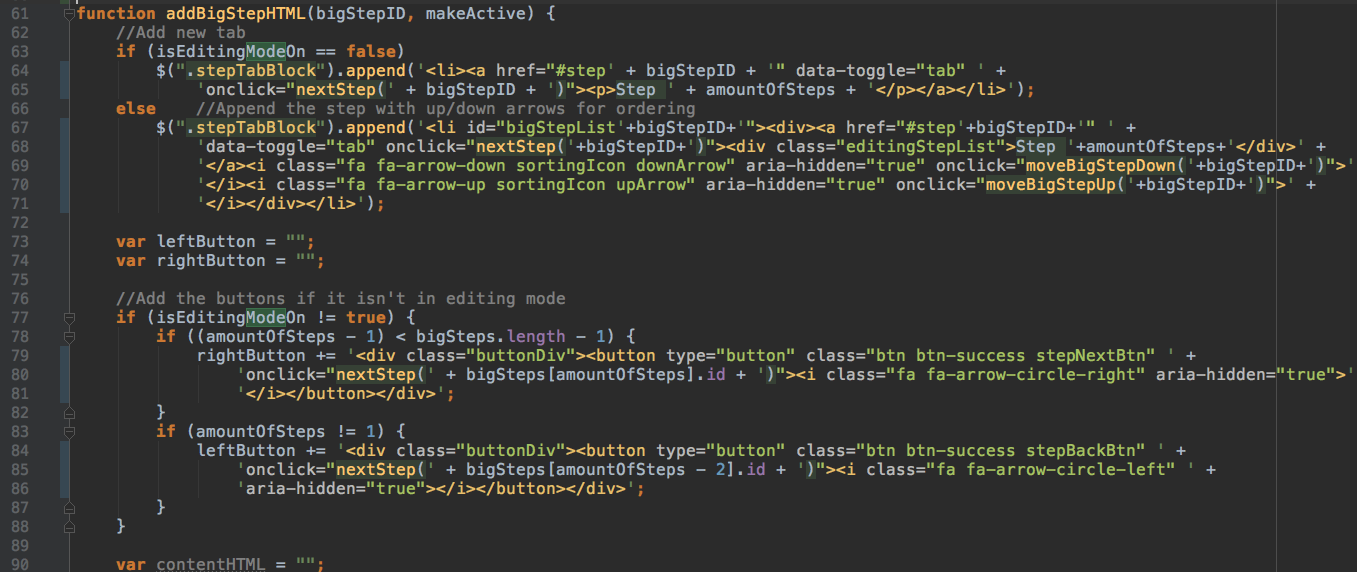
\includegraphics[width=1\linewidth]{images/stepsEdit&Present.png}
\caption{Show or Edit Steps Control Structure.}
\label{fig:edit_present_steps.}
\end{figure}	

 












